\chapter{Genomes of Cells and Viruses}\label{ch:b1:genomes}

Two metres of \omterm{def:b1:nucleic-acids:chain}{DNA} are folded into a nucleus six micrometres across,
and folded so that any of twenty thousand \omterm{def:b1:genomes:gene}{genes} can be found and read
within minutes. A bacterium folds a millimetre and a half into a \omterm{def:b1:cell-unit-of-life:cell}{cell}
a thousand times shorter, and copies it every twenty minutes. A \omterm{def:b1:genomes:virus}{virus}
carries a few thousand letters in a \omterm{def:b1:proteins:peptide}{protein} shell and reads them with
a \omterm{def:b1:cell-unit-of-life:cell}{cell} it does not own. This chapter describes the \emph{\omterm{def:b1:genomes:genome}{genome}} ---
the whole of an \omterm{def:b1:organism-environment:organism}{organism}'s \omterm{def:b1:nucleic-acids:chain}{DNA} --- as a physical object: how the \omterm{def:b1:nucleic-acids:chain}{DNA} of
bacteria, of \omterm{def:b1:cell-unit-of-life:prokeuk}{eukaryotic cells}, of \omterm{def:b1:cell-unit-of-life:prokeuk}{organelles} and of \omterm{def:b1:genomes:virus}{viruses} is
organised, what it contains besides \omterm{def:b1:genomes:gene}{genes}, and why the amount of it
says so little about the \omterm{def:b1:organism-environment:organism}{organism} that carries it.

\section{The bacterial genome}

\begin{definition}[Genome, chromosome, nucleoid]\label{def:b1:genomes:genome}
The \emph{genome}\index{genome} of a \omterm{def:b1:cell-unit-of-life:cell}{cell} is the totality of its \omterm{def:b1:nucleic-acids:chain}{DNA}:
the information for every \omterm{def:b1:proteins:peptide}{protein} and \omterm{def:b1:nucleic-acids:chain}{RNA} it can make, and the
sequences that control when they are made. A \emph{chromosome}\index{chromosome}
is one \omterm{def:b1:nucleic-acids:chain}{DNA} molecule with the \omterm{def:b1:proteins:peptide}{proteins} that organise it. A bacterium
usually has one, circular, of one to ten million \omterm{thm:b1:nucleic-acids:helix}{base pairs}
(\emph{E. coli}: $\num{4.6e6}$, \qty{1.5}{mm} long), folded into a
region of the \omterm{def:b1:cell-unit-of-life:cell}{cytoplasm}, the \emph{nucleoid}\index{nucleoid}, with no
membrane around it. Besides the chromosome many bacteria carry
\emph{plasmids}\index{plasmid}: small circles of a few thousand to a
few hundred thousand pairs, in one to hundreds of copies, replicating
on their own and carrying optional \omterm{def:b1:genomes:gene}{genes} --- antibiotic resistance,
toxins, the machinery for transferring themselves to another \omterm{def:b1:cell-unit-of-life:cell}{cell}.
\end{definition}

\begin{proposition}[How a bacterium folds its chromosome]\label{prop:b1:genomes:supercoiling}
\index{supercoiling}
A circular \omterm{def:b1:nucleic-acids:chain}{DNA} whose ends cannot rotate can be twisted like a rubber
band: \emph{supercoiling}. \omterm{def:b1:enzymes:enzyme}{Enzymes} called \emph{topoisomerases} cut,
pass and reseal the strands to add or remove turns; \emph{gyrase} uses
\omterm{def:b1:water-small-molecules:atp}{ATP} to introduce negative supercoils, which underwind the helix and
make it both more compact and easier to open. The \omterm{def:b1:genomes:genome}{chromosome} of
\emph{E. coli} is organised into some fifty loops, each supercoiled
independently and anchored to a \omterm{def:b1:proteins:peptide}{protein} core, so that the
\qty{1.5}{mm} occupies a \omterm{def:b1:genomes:genome}{nucleoid} of about a micrometre --- a
thousandfold compaction --- while any loop can be unwound for reading
or copying without disturbing the rest. Small basic \omterm{def:b1:proteins:peptide}{proteins}
(histone-like, though unrelated to \omterm{def:b1:genomes:nucleosome}{histones}) bend and bridge the \omterm{def:b1:nucleic-acids:chain}{DNA}
throughout.
\end{proposition}

\begin{omfigure}
\begin{tikzpicture}[font=\footnotesize, line cap=round]
  % relaxed circle
  \draw[very thick, omDef] (0,0) circle (1.1);
  \node[anchor=north, align=center] at (0,-1.35) {relaxed circle\\ (10.5 bp per turn)};
  % supercoiled: figure-eight / plectoneme
  \draw[very thick, omDef, domain=0:360, samples=240, smooth, variable=\t] plot ({4.3+1.05*cos(\t)}, {0.32*sin(4*\t)});
  \node[anchor=north, align=center] at (4.3,-1.35) {negatively supercoiled:\\ underwound, compact};
  \draw[->, thick] (1.35,0.15) -- (3.1,0.15) node[midway, above, align=center] {gyrase (ATP)};
  \draw[->, thick] (3.1,-0.25) -- (1.35,-0.25) node[midway, below, align=center] {topoisomerase I};
  % looped nucleoid
  \fill[omProp!40] (8.7,0) circle (0.35);
  \foreach \a in {0,45,...,315} {
    \draw[very thick, omDef] (8.7,0) .. controls ({8.7+1.6*cos(\a-20)},{1.6*sin(\a-20)}) and ({8.7+1.6*cos(\a+20)},{1.6*sin(\a+20)}) .. (8.7,0);
  }
  \node[anchor=north, align=center] at (8.7,-1.35) {the nucleoid: about fifty\\ supercoiled loops on a protein core};
\end{tikzpicture}

{\small A circular \omterm{def:b1:genomes:genome}{chromosome} relaxed, supercoiled, and organised
into loops. Supercoiling compacts the molecule and stores the energy
that helps open it; the loops let one region be unwound at a time.}
\end{omfigure}

\begin{example}[A dense genome]\label{ex:b1:genomes:dense}
Of the \emph{E. coli} \omterm{def:b1:genomes:genome}{chromosome}'s \qty{4.6}{Mb}, \qty{88}{\%} codes
for \omterm{def:b1:proteins:peptide}{protein}: some \num{4300} \omterm{def:b1:genomes:gene}{genes} of about \num{1000} pairs each,
packed head to tail with a hundred pairs between them, many grouped
into \emph{operons} transcribed together (\cref{ch:b1:expression-control}).
A \omterm{def:b1:genomes:genome}{plasmid} of \qty{5}{kb} may carry three \omterm{def:b1:genomes:gene}{genes} and exist in fifty
copies; the resistance \omterm{def:b1:genomes:gene}{gene} it carries can spread through a hospital
ward's bacteria in weeks, by conjugation, faster than any mutation
could arise.
\end{example}

\section{The eukaryotic genome: chromatin}

\begin{definition}[Nucleosome, chromatin]\label{def:b1:genomes:nucleosome}
\index{nucleosome}\index{histone}\index{chromatin}
In a eukaryotic nucleus the \omterm{def:b1:nucleic-acids:chain}{DNA} is wound on \omterm{def:b1:proteins:peptide}{proteins}: \qty{147}{} \omterm{thm:b1:nucleic-acids:helix}{base
pairs} make 1.7 turns around an octamer of eight \emph{histones}
(two each of H2A, H2B, H3, H4, small \omterm{def:b1:proteins:peptide}{proteins} rich in lysine and
arginine that neutralise the phosphates), forming a
\emph{nucleosome}\index{nucleosome} \qty{11}{nm} across; nucleosomes
follow one another every \qty{200}{} pairs or so, like beads on a
string, with a fifth histone, H1, sealing each bead. This
\emph{chromatin} folds further: into a fibre of \qty{30}{nm}, into
loops of tens of thousands of pairs anchored on a \omterm{def:b1:proteins:peptide}{protein} scaffold,
and --- at division --- into the compact rods of the metaphase
\omterm{def:b1:genomes:genome}{chromosome}, ten thousand times shorter than the naked \omterm{def:b1:nucleic-acids:chain}{DNA}.
\emph{Euchromatin} is the looser, gene-rich, transcribed form of
interphase; \emph{heterochromatin} the condensed, gene-poor form that
stays compact (around \omterm{def:b1:genomes:karyotype}{centromeres}, at the ends, and on a switched-off
X \omterm{def:b1:genomes:genome}{chromosome}).
\end{definition}

\begin{omfigure}
\begin{tikzpicture}[font=\footnotesize, >=Stealth, line cap=round]
  % level 1: double helix line
  \draw[very thick, omDef] (0,5.4) -- (3.2,5.4);
  \node[anchor=west, align=left] at (3.5,5.4) {double helix, \qty{2}{nm}};
  % level 2: beads on a string
  \draw[thick, omDef] (0,4.2) -- (3.2,4.2);
  \foreach \x in {0.4,1.2,2.0,2.8} { \fill[omProp!70] (\x,4.2) circle (0.22); \draw[thick, omDef] (\x,4.2) circle (0.3); }
  \node[anchor=west, align=left] at (3.5,4.2) {nucleosomes, \qty{11}{nm}: \qty{147}{bp} around a histone octamer,\\ every \qty{200}{bp} --- compaction $\times 6$};
  % level 3: 30 nm fibre (zigzag stack)
  \foreach \i in {0,...,9} { \fill[omProp!70] (0.2+0.3*\i,{3.0+0.18*(-1)^\i}) circle (0.17); }
  \node[anchor=west, align=left] at (3.5,3.0) {\qty{30}{nm} fibre: nucleosomes stacked --- $\times 40$};
  % level 4: loops on scaffold
  \draw[very thick, gray] (0,1.5) -- (3.2,1.5);
  \foreach \x in {0.4,1.2,2.0,2.8} { \draw[thick, omProp!80!black] (\x,1.5) .. controls (\x-0.35,2.3) and (\x+0.35,2.3) .. (\x,1.5); }
  \node[anchor=west, align=left] at (3.5,1.8) {loops of \qtyrange{50}{100}{kb} on a scaffold, \qty{300}{nm} --- $\times 1000$};
  % level 5: metaphase chromosome
  \draw[very thick, omThm, fill=omThm!30, rounded corners=4pt] (0.9,-0.3) rectangle (1.4,1.0);
  \draw[very thick, omThm, fill=omThm!30, rounded corners=4pt] (1.7,-0.3) rectangle (2.2,1.0);
  \fill[omThm!60!black] (1.55,0.45) ellipse (0.45 and 0.13);
  \node[anchor=west, align=left] at (3.5,0.35) {metaphase chromosome, \qty{1400}{nm} across: $\times \num{10000}$\\ (\qty{8.5}{cm} of DNA in \qty{10}{\micro m})};
\end{tikzpicture}

{\small Levels of packing of eukaryotic \omterm{def:b1:nucleic-acids:chain}{DNA}, from the helix to the
metaphase \omterm{def:b1:genomes:genome}{chromosome}. Each level multiplies the compaction; the whole
reaches ten thousand.}
\end{omfigure}

\begin{omfigure}
\begin{minipage}[b]{0.46\linewidth}\centering
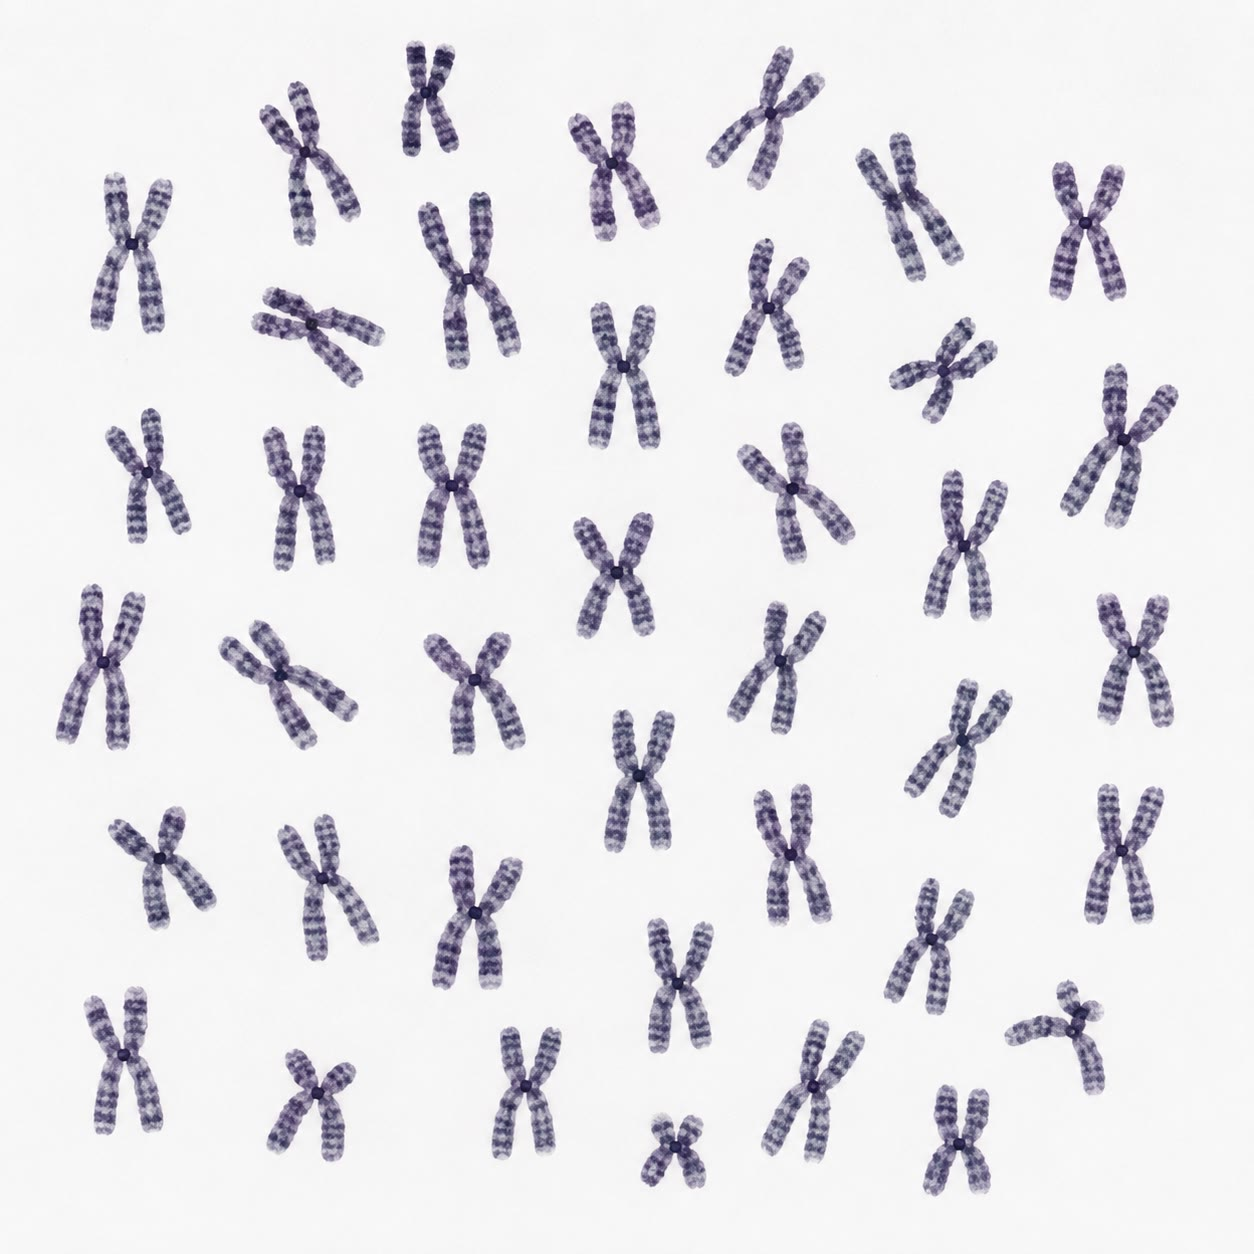
\includegraphics[width=0.94\linewidth]{images/book3/ai/b3-17-metaphase-spread.jpg}
\end{minipage}\hfill
\begin{minipage}[b]{0.5\linewidth}\centering
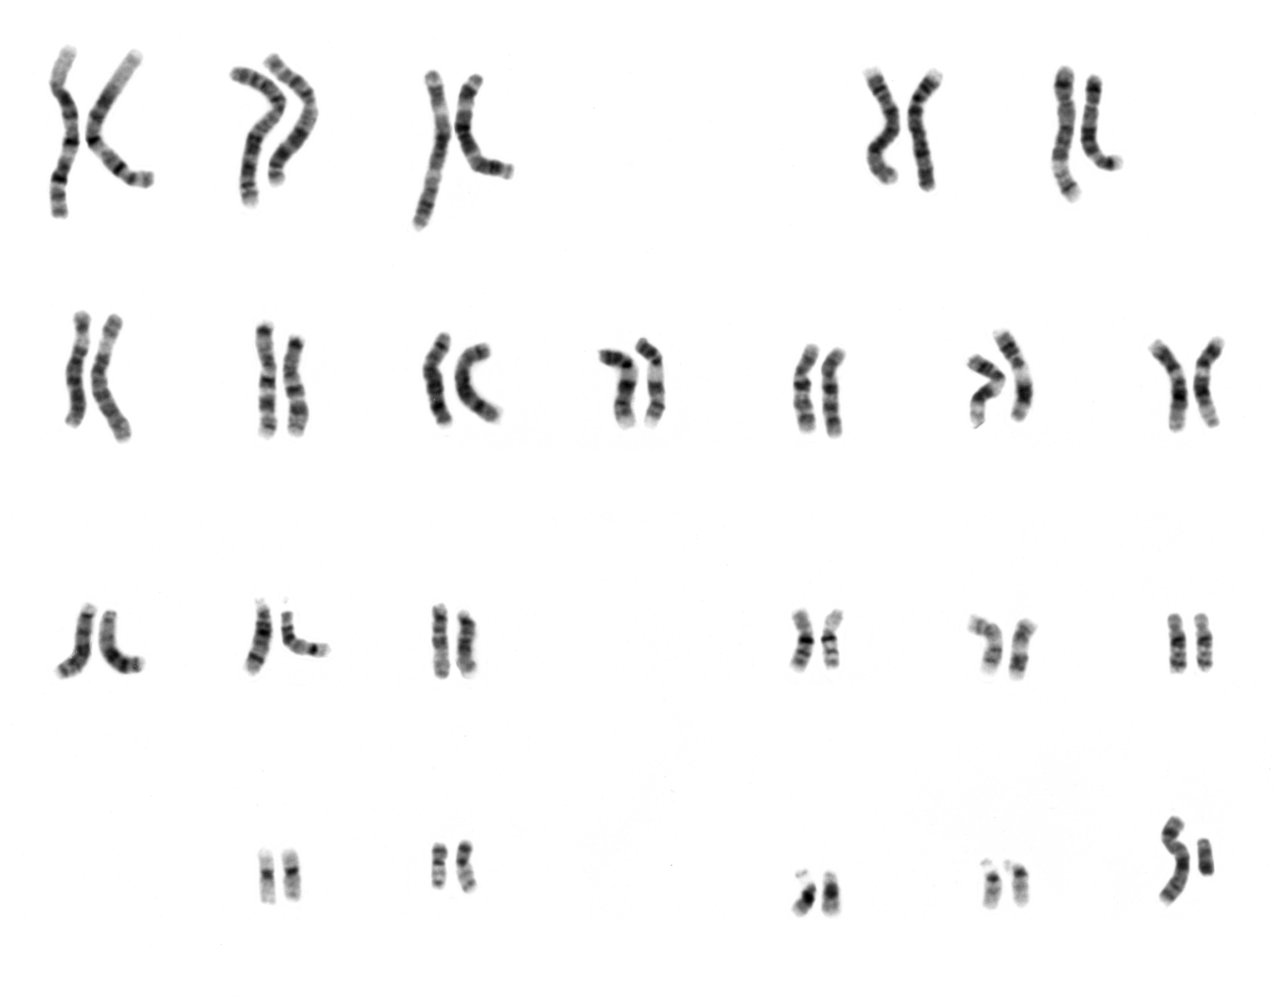
\includegraphics[width=0.96\linewidth]{images/book3/karyotype.png}
\end{minipage}

{\small Left: the \omterm{def:b1:genomes:genome}{chromosomes} of one human \omterm{def:b1:cell-unit-of-life:cell}{cell}, spread from a \omterm{def:b1:cell-unit-of-life:cell}{cell}
arrested at metaphase. Right: the same \omterm{def:b1:genomes:genome}{chromosomes} sorted by size and
banding into a \omterm{def:b1:genomes:karyotype}{karyotype} --- twenty-two pairs and XY, forty-six in all.
\omterm{def:b1:genomes:karyotype}{Karyotype}: National Human \omterm{def:b1:genomes:genome}{Genome} Research Institute, public domain.}
\end{omfigure}

\begin{definition}[Karyotype, centromere, telomere]\label{def:b1:genomes:karyotype}
\index{karyotype}\index{centromere}\index{telomere}
The \emph{karyotype} is the set of \omterm{def:b1:genomes:genome}{chromosomes} of a \omterm{def:b1:cell-unit-of-life:cell}{cell}, sorted by
size and banding pattern: humans have 23 pairs (22 autosomes and XY or
XX), $\num{6.4e9}$ \omterm{thm:b1:nucleic-acids:helix}{base pairs} in all, \qty{2.2}{m}; the largest
\omterm{def:b1:genomes:genome}{chromosome} holds \qty{250}{Mb}, the smallest \qty{50}{}. Each linear
\omterm{def:b1:genomes:genome}{chromosome} carries a \emph{centromere}, the constricted region where
the two copies stay joined after replication and where the spindle
attaches (\cref{ch:b1:replication-mitosis}), and two \emph{telomeres},
repeated sequences at the ends that protect them from being taken for
broken \omterm{def:b1:nucleic-acids:chain}{DNA} and from shortening at each replication.
\end{definition}

\begin{proposition}[Genome size does not measure complexity]\label{prop:b1:genomes:cvalue}
\index{C-value paradox}
\begin{center}
\small
\begin{tabular}{lrr}
\hline
\omterm{def:b1:organism-environment:organism}{organism} & \omterm{def:b1:genomes:genome}{genome} (Mb) & protein-coding \omterm{def:b1:genomes:gene}{genes} \\
\hline
\emph{E. coli} & 4.6 & \num{4300} \\
yeast & 12 & \num{6000} \\
fruit fly & 140 & \num{14000} \\
human & 3200 & \num{20000} \\
maize & 2300 & \num{40000} \\
lungfish & \num{130000} & $\approx\num{20000}$ \\
\emph{Paris japonica} (a lily) & \num{150000} & $\approx\num{30000}$ \\
\hline
\end{tabular}
\end{center}
\omterm{def:b1:genomes:genome}{Genome} size varies a thousandfold among eukaryotes with no relation to
the number of \omterm{def:b1:genomes:gene}{genes} or the complexity of the \omterm{def:b1:organism-environment:organism}{organism} (the
\emph{C-value paradox}): a lungfish carries forty times the \omterm{def:b1:nucleic-acids:chain}{DNA} of a
human and no more \omterm{def:b1:genomes:gene}{genes}. The difference is not \omterm{def:b1:genomes:gene}{genes} but the \omterm{def:b1:nucleic-acids:chain}{DNA}
between them.
\end{proposition}

\section{What a genome contains}

\begin{definition}[Anatomy of a gene]\label{def:b1:genomes:gene}
\index{gene}\index{exon}\index{intron}\index{promoter}
A \emph{gene} is a stretch of \omterm{def:b1:nucleic-acids:chain}{DNA} transcribed into a functional \omterm{def:b1:nucleic-acids:chain}{RNA}
--- usually a messenger for one \omterm{def:b1:proteins:peptide}{protein}. A eukaryotic protein-coding
gene comprises a \emph{promoter}, the sequence upstream where
transcription begins and is controlled; \emph{exons}, the parts kept
in the mature message; \emph{introns}, the parts transcribed and then
cut out (\cref{ch:b1:gene-expression}); the untranslated regions at
each end of the message; and a terminator. A human gene averages
\qty{27}{kb} with eight exons totalling \qty{1.5}{kb}: nineteen
twentieths of a typical gene is intron. Bacterial genes have no
introns.
\end{definition}

\begin{omfigure}
\begin{tikzpicture}[font=\footnotesize, >=Stealth, line cap=round]
  \draw[very thick, gray] (0,0) -- (12.6,0);
  \fill[omExo!50] (0.2,-0.18) rectangle (1.6,0.18); \node[anchor=north] at (0.9,-0.25) {promoter};
  \fill[omDef!70] (1.6,-0.25) rectangle (2.4,0.25);
  \fill[omDef!70] (4.6,-0.25) rectangle (5.6,0.25);
  \fill[omDef!70] (8.4,-0.25) rectangle (9.0,0.25);
  \fill[omDef!70] (10.9,-0.25) rectangle (12.0,0.25);
  \node[anchor=south, omDef!70!black] at (2.0,0.3) {exon 1};
  \node[anchor=south, omDef!70!black] at (5.1,0.3) {exon 2};
  \node[anchor=south, omDef!70!black] at (8.7,0.3) {exon 3};
  \node[anchor=south, omDef!70!black] at (11.45,0.3) {exon 4};
  \node[anchor=north] at (3.5,-0.3) {intron 1};
  \node[anchor=north] at (7.0,-0.3) {intron 2};
  \node[anchor=north] at (9.95,-0.3) {intron 3};
  \draw[->, thick, omExo!70!black] (1.6,0.75) -- (2.6,0.75); \node[anchor=south, font=\scriptsize] at (2.6,0.85) {transcription starts here};
  \node[anchor=north, align=center, gray] at (6.3,-0.9) {a typical human gene: \qty{27}{kb} of which \qty{1.5}{kb} of exons;\\ the exons are joined in the mature messenger, the introns discarded};
\end{tikzpicture}

{\small A eukaryotic \omterm{def:b1:genomes:gene}{gene}: a \omterm{def:b1:genomes:gene}{promoter}, \omterm{def:b1:genomes:gene}{exons} (kept) alternating with
\omterm{def:b1:genomes:gene}{introns} (removed after transcription). Drawn to a compressed scale ---
in a real \omterm{def:b1:genomes:gene}{gene} the \omterm{def:b1:genomes:gene}{introns} would be twenty times longer than the \omterm{def:b1:genomes:gene}{exons}.}
\end{omfigure}

\begin{proposition}[The census of the human genome]\label{prop:b1:genomes:census}
\index{transposon}\index{repeated DNA}
Of the \qty{3.2}{Gb}: about \qty{1.5}{\%} codes for \omterm{def:b1:proteins:peptide}{protein}; \qty{25}{\%}
is \omterm{def:b1:genomes:gene}{intron}; \qty{45}{\%} is the remains of \emph{transposable elements}
--- sequences that copy themselves into new places, mostly long dead
(the Alu element alone, \qty{300}{bp}, is present in a million copies,
a tenth of the \omterm{def:b1:genomes:genome}{genome}); \qty{8}{\%} is short repeats in tandem
(satellite \omterm{def:b1:nucleic-acids:chain}{DNA}, at \omterm{def:b1:genomes:karyotype}{centromeres} and \omterm{def:b1:genomes:karyotype}{telomeres}); the rest is unique
non-coding sequence that includes the \omterm{def:b1:genomes:gene}{promoters}, enhancers and \omterm{def:b1:nucleic-acids:chain}{RNA}
\omterm{def:b1:genomes:gene}{genes} that control expression. Many \omterm{def:b1:genomes:gene}{genes} belong to \emph{families}
that arose by duplication (the globins, the olfactory receptors ---
a thousand of them), and the \omterm{def:b1:genomes:genome}{genome} holds thousands of
\emph{pseudogenes}, dead copies that no longer work. A \omterm{def:b1:genomes:genome}{genome} is not
a design but a record.
\end{proposition}

\begin{omfigure}
\begin{tikzpicture}[font=\footnotesize]
  \def\R{2.1}
  % slices: coding 1.5, introns 25, transposons 45, satellite 8, other 20.5
  \fill[omThm!70] (0,0) -- (90:\R) arc (90:84.6:\R) -- cycle;
  \fill[omDef!50] (0,0) -- (84.6:\R) arc (84.6:-5.4:\R) -- cycle;
  \fill[omProp!50] (0,0) -- (-5.4:\R) arc (-5.4:-167.4:\R) -- cycle;
  \fill[omExo!50] (0,0) -- (-167.4:\R) arc (-167.4:-196.2:\R) -- cycle;
  \fill[gray!30] (0,0) -- (-196.2:\R) arc (-196.2:-270:\R) -- cycle;
  \draw[thick] (0,0) circle (\R);
  \node[anchor=west, omThm!80!black] at (0.3,2.35) {protein-coding exons \qty{1.5}{\%}};
  \draw[omThm!80!black] (87:\R) -- (0.3,2.35);
  \node[anchor=west] at (2.3,0.9) {introns \qty{25}{\%}};
  \node[anchor=north] at (0,-2.3) {transposable elements and their remains \qty{45}{\%}};
  \node[anchor=east] at (-2.3,-0.4) {satellite repeats \qty{8}{\%}};
  \node[anchor=east] at (-2.3,1.2) {other unique DNA \qty{20}{\%}};
\end{tikzpicture}

{\small What the human \omterm{def:b1:genomes:genome}{genome} is made of. The \omterm{def:b1:genomes:gene}{exons} that code for
\omterm{def:b1:proteins:peptide}{protein} are a sliver; half the \omterm{def:b1:genomes:genome}{genome} is the debris of elements that
once copied themselves.}
\end{omfigure}

\begin{example}[Reading a genome's size]\label{ex:b1:genomes:sizes}
A \omterm{def:b1:genomes:genome}{genome} of \qty{4.6}{Mb} with no \omterm{def:b1:genomes:gene}{introns} and few repeats holds
\num{4300} \omterm{def:b1:genomes:gene}{genes}; one of \qty{3200}{Mb} with long \omterm{def:b1:genomes:gene}{introns} and half
its length in repeats holds \num{20000}; one of \qty{130000}{Mb} holds
the same twenty thousand. The size measures how much has accumulated
in a lineage's non-coding \omterm{def:b1:nucleic-acids:chain}{DNA}, and how efficiently it has been
removed, not how much the \omterm{def:b1:organism-environment:organism}{organism} does.
\end{example}

\section{Organelle genomes and viruses}

\begin{definition}[Organelle genomes]\label{def:b1:genomes:organelle}
\omterm{def:b1:eukaryotic-cell:mitochondrion}{Mitochondria} and \omterm{def:b1:eukaryotic-cell:plastid}{chloroplasts} keep a remnant of their bacterial
ancestors' \omterm{def:b1:genomes:genome}{chromosome} (\cref{ch:b1:eukaryotic-cell}): a small circle
--- \qty{16.6}{kb} and 37 \omterm{def:b1:genomes:gene}{genes} in human \omterm{def:b1:eukaryotic-cell:mitochondrion}{mitochondria}, \qtyrange{120}{160}{kb}
and about 100 \omterm{def:b1:genomes:gene}{genes} in \omterm{def:b1:eukaryotic-cell:plastid}{chloroplasts} --- in many copies per \omterm{def:b1:cell-unit-of-life:prokeuk}{organelle},
coding for some of their own \omterm{def:b1:proteins:peptide}{proteins} and for the \omterm{def:b1:nucleic-acids:chain}{RNAs} of their
ribosomes. The rest of their \omterm{def:b1:proteins:peptide}{proteins} come from nuclear \omterm{def:b1:genomes:gene}{genes}. In most
animals the mitochondrial \omterm{def:b1:genomes:genome}{genome} is inherited from the mother only,
with the egg's \omterm{def:b1:cell-unit-of-life:cell}{cytoplasm}.
\end{definition}

\begin{definition}[Virus]\label{def:b1:genomes:virus}
\index{virus}\index{capsid}
A \emph{virus} is a \omterm{def:b1:genomes:genome}{genome} in a \omterm{def:b1:proteins:peptide}{protein} shell, the \emph{capsid} ---
sometimes wrapped in a membrane, the \emph{envelope}, taken from a
host \omterm{def:b1:cell-unit-of-life:cell}{cell} --- that reproduces only inside a \omterm{def:b1:cell-unit-of-life:cell}{cell}, using the \omterm{def:b1:cell-unit-of-life:cell}{cell}'s
ribosomes, energy and precursors. Its \omterm{def:b1:genomes:genome}{genome} may be \omterm{def:b1:nucleic-acids:chain}{DNA} or \omterm{def:b1:nucleic-acids:chain}{RNA},
double- or single-stranded, linear or circular, one molecule or
several: from \qty{5}{kb} (a few \omterm{def:b1:genomes:gene}{genes}) to \qty{1.2}{Mb} (a thousand,
in the giant viruses). Outside a \omterm{def:b1:cell-unit-of-life:cell}{cell} a virus does nothing: it is not
a \omterm{def:b1:cell-unit-of-life:cell}{cell}, does not metabolise, and is alive only in the sense that it
carries information and evolves. The \emph{bacteriophages} are the
viruses of bacteria.
\end{definition}

\begin{omfigure}
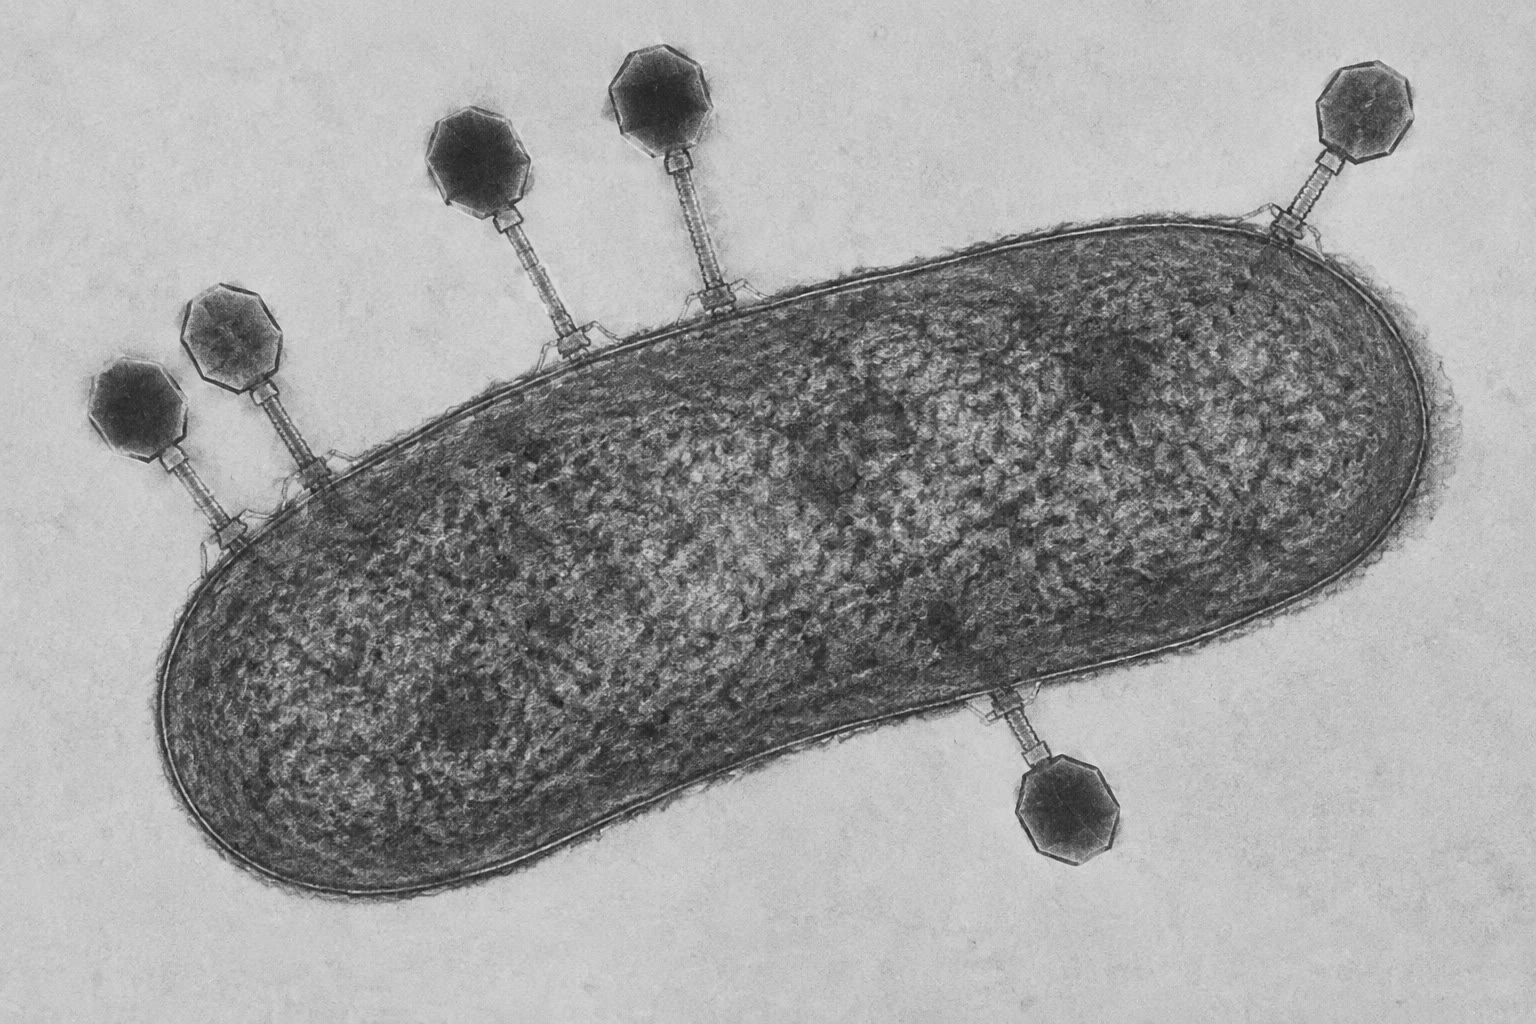
\includegraphics[width=0.5\linewidth]{images/book3/ai/b3-17-phage-on-bacterium.jpg}

{\small Bacteriophages attached to a bacterium: polyhedral heads
holding the \omterm{def:b1:nucleic-acids:chain}{DNA}, tails through which it will be injected. A single
\omterm{def:b1:cell-unit-of-life:cell}{cell} will release a hundred new phages within half an hour.}
\end{omfigure}

\begin{proposition}[The two cycles of phage $\lambda$]\label{prop:b1:genomes:lambda}
\index{lytic cycle}\index{lysogenic cycle}
Phage $\lambda$ injects its \qty{48.5}{kb} of \omterm{def:b1:nucleic-acids:chain}{DNA} (\cref{ch:b1:nucleic-acids})
into \emph{E. coli}, where it circularises. Two \omterm{def:b1:lipids:triglyceride}{fates} follow. In the
\emph{\omterm{prop:b1:genomes:lambda}{lytic cycle}} the phage's \omterm{def:b1:genomes:gene}{genes} are transcribed by the host's
polymerase, its \omterm{def:b1:nucleic-acids:chain}{DNA} is replicated a hundredfold, \omterm{def:b1:genomes:virus}{capsid} \omterm{def:b1:proteins:peptide}{proteins} are
made and assembled, the \omterm{def:b1:nucleic-acids:chain}{DNA} is packed into them, and an \omterm{def:b1:enzymes:enzyme}{enzyme}
dissolves the wall: the \omterm{def:b1:cell-unit-of-life:cell}{cell} bursts, releasing a hundred phages, forty
minutes after infection. In the \emph{\omterm{prop:b1:genomes:lambda}{lysogenic cycle}} the phage \omterm{def:b1:nucleic-acids:chain}{DNA}
is inserted into the host \omterm{def:b1:genomes:genome}{chromosome} and silenced by a repressor of
its own making: the \emph{prophage} is copied with the \omterm{def:b1:genomes:genome}{chromosome} for
generations, invisible, until damage to the host's \omterm{def:b1:nucleic-acids:chain}{DNA} lifts the
repression and the \omterm{prop:b1:genomes:lambda}{lytic cycle} resumes. The choice is a molecular
switch, one of the first understood (\cref{ch:b1:expression-control}).
\end{proposition}

\begin{omfigure}
\begin{tikzpicture}[font=\footnotesize, >=Stealth, line cap=round,
  st/.style={draw, thick, rounded corners=3pt, inner sep=3pt, align=center, fill=white}]
  \node[st, fill=omDef!12] (inj) at (0,0) {phage DNA injected,\\ circularised};
  \node[st, fill=omThm!12] (rep) at (4.6,1.4) {replication, capsid\\ proteins, assembly};
  \node[st, fill=omThm!12] (lys) at (9.2,1.4) {lysis: \qty{100}{} phages\\ released, \qty{40}{min}};
  \node[st, fill=omExo!12] (pro) at (4.6,-1.4) {integrated as a prophage,\\ silenced by its repressor};
  \node[st, fill=omExo!12] (div) at (9.2,-1.4) {copied with the host\\ chromosome for generations};
  \draw[->, thick, omThm] (inj) -- (rep) node[pos=0.45, above left, omThm] {lytic};
  \draw[->, thick, omThm] (rep) -- (lys);
  \draw[->, thick, omExo!70!black] (inj) -- (pro) node[pos=0.4, below left, omExo!70!black] {lysogenic};
  \draw[->, thick, omExo!70!black] (pro) -- (div);
  \draw[->, thick, dashed, gray] (div.north) -- (lys.south) node[midway, right, align=left, font=\scriptsize] {induction\\ (host DNA damaged)};
\end{tikzpicture}

{\small Phage $\lambda$: \omterm{prop:b1:genomes:lambda}{lytic cycle} (red) or lysogenic (green), and
the induction that turns the second into the first.}
\end{omfigure}

\begin{example}[Viruses with RNA genomes]\label{ex:b1:genomes:rna}
Influenza carries eight segments of single-stranded \omterm{def:b1:nucleic-acids:chain}{RNA} and its own
polymerase to copy them, since \omterm{def:b1:cell-unit-of-life:cell}{cells} have no \omterm{def:b1:enzymes:enzyme}{enzyme} that copies \omterm{def:b1:nucleic-acids:chain}{RNA};
its polymerase makes one error per \num{10000} bases and the \omterm{def:b1:genomes:virus}{virus}
changes every season. A retrovirus (HIV) carries \omterm{def:b1:nucleic-acids:chain}{RNA} and a
\emph{reverse transcriptase} that copies it into \omterm{def:b1:nucleic-acids:chain}{DNA}, which is inserted
into the host \omterm{def:b1:genomes:genome}{chromosome} like a prophage --- a permanent infection.
The mechanisms, and the immune response to them, are the Year 3
volume's; here they mark the range of what a \omterm{def:b1:genomes:genome}{genome} can be.
\end{example}

\section{Exercises}

\begin{exercise}[$\star$]\label{exo:b1:genomes:1}
Compare the bacterial and the eukaryotic \omterm{def:b1:genomes:genome}{genome}: number and shape of
the \omterm{def:b1:genomes:genome}{chromosomes}, location, \omterm{def:b1:proteins:peptide}{proteins} that organise them, and \omterm{def:b1:genomes:gene}{gene}
density.
\end{exercise}

\begin{exercise}[$\star$]\label{exo:b1:genomes:2}
Describe a \omterm{def:b1:genomes:nucleosome}{nucleosome} and give the compaction factor of each level of
\omterm{def:b1:genomes:nucleosome}{chromatin} folding.
\end{exercise}

\begin{exercise}[$\star$]\label{exo:b1:genomes:3}
From the census figure, what fraction of the human \omterm{def:b1:genomes:genome}{genome} codes for
\omterm{def:b1:proteins:peptide}{protein}, and what is the largest category?
\end{exercise}

\begin{exercise}[$\star$]\label{exo:b1:genomes:4}
What is a \omterm{def:b1:genomes:virus}{virus}, and in what sense is it not alive?
\end{exercise}

\begin{exercise}[$\star\star$]\label{exo:b1:genomes:5}
Compute the length of the \emph{E. coli} \omterm{def:b1:genomes:genome}{chromosome} and the number of
nucleosome-sized turns it would need if it were eukaryotic; explain
how the bacterium compacts it instead.
\end{exercise}

\begin{exercise}[$\star\star$]\label{exo:b1:genomes:6}
A human \omterm{def:b1:genomes:gene}{gene} of \qty{27}{kb} has \qty{1.5}{kb} of \omterm{def:b1:genomes:gene}{exons} in eight
pieces. Compute the mean \omterm{def:b1:genomes:gene}{exon} and \omterm{def:b1:genomes:gene}{intron} lengths and the fraction of
the primary transcript that is discarded.
\end{exercise}

\begin{exercise}[$\star\star$]\label{exo:b1:genomes:7}
Using the table, compute the \omterm{def:b1:genomes:gene}{genes} per megabase for \emph{E. coli},
yeast, the fruit fly, the human and the lungfish. Comment on the trend.
\end{exercise}

\begin{exercise}[$\star\star$]\label{exo:b1:genomes:8}
The Alu element is \qty{300}{bp} and present in a million copies.
What fraction of the \omterm{def:b1:genomes:genome}{genome} is Alu? If each copy arose by
retrotransposition (an \omterm{def:b1:nucleic-acids:chain}{RNA} copied back to \omterm{def:b1:nucleic-acids:chain}{DNA} and inserted), how many
insertions per generation would produce a million copies in
\num{60} million years at \num{20} years a generation?
\end{exercise}

\begin{exercise}[$\star\star$]\label{exo:b1:genomes:9}
Explain why the mitochondrial \omterm{def:b1:genomes:genome}{genome} is inherited maternally, and
what this implies for tracing ancestry.
\end{exercise}

\begin{exercise}[$\star\star\star$]\label{exo:b1:genomes:10}
Phage $\lambda$ in the lysogenic state is copied once per host
generation; in the lytic state it makes a hundred copies in
\qty{40}{min}. In a well-fed culture doubling every \qty{20}{min},
compare the two strategies over two hours; in a starving culture that
does not divide, compare them again. Why does the switch respond to
the host's condition?
\end{exercise}

\begin{exercise}[$\star\star\star$]\label{exo:b1:genomes:11}
A lungfish \omterm{def:b1:cell-unit-of-life:cell}{cell} carries \qty{130}{Gb}: compute the \omterm{def:b1:nucleic-acids:chain}{DNA} length, the
number of \omterm{def:b1:genomes:nucleosome}{nucleosomes} and the mass of \omterm{def:b1:genomes:nucleosome}{histones} per \omterm{def:b1:cell-unit-of-life:cell}{cell}, and the time
to replicate it at the human fork speed (\qty{50}{bp/s} per fork) with
one origin per \qty{100}{kb}. What does a large \omterm{def:b1:genomes:genome}{genome} cost a \omterm{def:b1:cell-unit-of-life:cell}{cell}?
\end{exercise}

\begin{exercise}[$\star\star\star$]\label{exo:b1:genomes:12}
``The \omterm{def:b1:genomes:genome}{genome} is a record, not a design.'' Discuss in a paragraph with
pseudogenes, transposable elements, \omterm{def:b1:genomes:gene}{gene} families and the C-value
paradox.
\end{exercise}

\section{Problem: Two Metres in Six Micrometres}

\begin{problem}[{Weekend problem --- a human nucleus measured from the
helix to the chromosome: lengths, volumes, nucleosomes, histones and
the packing ratio at every level, ending on the total compaction of
metaphase}]
\label{pb:b1:genomes:1}
A human diploid nucleus is a sphere of \qty{6}{\micro m} diameter
holding $\num{6.4e9}$ \omterm{thm:b1:nucleic-acids:helix}{base pairs} on 46 \omterm{def:b1:genomes:genome}{chromosomes}; the largest
\omterm{def:b1:genomes:genome}{chromosome} carries \qty{250}{Mb}, the smallest \qty{50}{}. Take
\qty{0.34}{nm} per pair, \qty{2}{nm} for the helix diameter,
\qty{650}{Da} per pair, \num{200} pairs per \omterm{def:b1:genomes:nucleosome}{nucleosome}, a \omterm{def:b1:genomes:nucleosome}{histone}
octamer of \qty{108}{kDa}, and $\qty{1.66e-24}{g}$ per dalton.

\medskip
\noindent\textbf{Part I --- Lengths and volumes.}
\begin{enumerate}
  \item Compute the total length of \omterm{def:b1:nucleic-acids:chain}{DNA} in the nucleus.
  \item Compute the number of turns of the \omterm{thm:b1:nucleic-acids:helix}{double helix} it contains.
  \item Compute the length of the largest and of the smallest
        \omterm{def:b1:genomes:genome}{chromosome}'s \omterm{def:b1:nucleic-acids:chain}{DNA}.
  \item Compute the volume of the nucleus.
  \item Compute the volume of the \omterm{def:b1:nucleic-acids:chain}{DNA} as a cylinder, and the fraction
        of the nucleus it occupies.
  \item Compute the mass of \omterm{def:b1:nucleic-acids:chain}{DNA} in the nucleus in picograms.
  \item The nucleus contains about \qty{25}{pg} of \omterm{def:b1:proteins:peptide}{protein}. What
        fraction of the nuclear mass is \omterm{def:b1:nucleic-acids:chain}{DNA}, if water is \qty{80}{\%}
        of the nucleus (density \qty{1.1}{g/mL})?
\end{enumerate}

\medskip
\noindent\textbf{Part II --- \omterm{def:b1:genomes:nucleosome}{Nucleosomes}.}
\begin{enumerate}[resume]
  \item Compute the number of \omterm{def:b1:genomes:nucleosome}{nucleosomes} in the nucleus.
  \item Compute the mass of \omterm{def:b1:genomes:nucleosome}{histones} and compare with the mass of
        \omterm{def:b1:nucleic-acids:chain}{DNA}.
  \item The \qty{200}{} pairs of one \omterm{def:b1:genomes:nucleosome}{nucleosome} span \qty{68}{nm} of
        helix but occupy a bead \qty{11}{nm} long. Compute the
        compaction factor of the ``beads on a string''.
  \item The \qty{30}{nm} fibre holds six \omterm{def:b1:genomes:nucleosome}{nucleosomes} per \qty{11}{nm}
        of its length. Compute its compaction factor relative to naked
        \omterm{def:b1:nucleic-acids:chain}{DNA}.
  \item Compute the length of the \qty{30}{nm} fibre for the whole
        \omterm{def:b1:genomes:genome}{genome}, and compare it with the nucleus's diameter.
  \item Each \omterm{def:b1:genomes:nucleosome}{nucleosome} must be taken apart and reassembled when the
        \omterm{def:b1:nucleic-acids:chain}{DNA} is replicated or transcribed. How many \omterm{def:b1:genomes:nucleosome}{nucleosomes} are
        reassembled in S phase (\qty{8}{h})? Per second?
\end{enumerate}

\medskip
\noindent\textbf{Part III --- Loops and \omterm{def:b1:genomes:genome}{chromosomes}.}
\begin{enumerate}[resume]
  \item Loops of \qty{75}{kb} of the \qty{30}{nm} fibre hang from a
        scaffold. Compute the length of fibre in one loop and the
        number of loops in the \omterm{def:b1:genomes:genome}{genome}.
  \item A metaphase chromatid of the largest \omterm{def:b1:genomes:genome}{chromosome} is
        \qty{10}{\micro m} long. Compute the compaction factor from
        naked \omterm{def:b1:nucleic-acids:chain}{DNA} to metaphase \omterm{def:b1:genomes:genome}{chromosome}.
  \item Compute the volume of that chromatid as a cylinder of
        \qty{0.7}{\micro m} diameter, and the fraction of it that is
        \omterm{def:b1:nucleic-acids:chain}{DNA}.
  \item The 46 \omterm{def:b1:genomes:genome}{chromosomes} at metaphase, each a rod of the same
        density: compute their total volume and compare it with the
        interphase nucleus.
  \item Explain why interphase \omterm{def:b1:genomes:nucleosome}{chromatin} cannot be packed as tightly
        as metaphase \omterm{def:b1:genomes:nucleosome}{chromatin}.
\end{enumerate}

\medskip
\noindent\textbf{Part IV --- Finding a \omterm{def:b1:genomes:gene}{gene}.}
\begin{enumerate}[resume]
  \item A \omterm{def:b1:proteins:peptide}{protein} must find one \qty{20}{bp} site in the \omterm{def:b1:genomes:genome}{genome}.
        If it tested one random site per millisecond, how long would
        the search take? What does this say about how sites are
        found?
  \item The \omterm{def:b1:genomes:genome}{genome}'s \qty{20000}{} \omterm{def:b1:genomes:gene}{genes} average \qty{27}{kb}. What
        fraction of the \omterm{def:b1:genomes:genome}{genome} is inside \omterm{def:b1:genomes:gene}{genes}? What fraction is
        coding, at \qty{1.5}{kb} of \omterm{def:b1:genomes:gene}{exons} per \omterm{def:b1:genomes:gene}{gene}?
  \item Each \omterm{def:b1:genomes:genome}{chromosome} occupies its own territory of the nucleus.
        Compute the volume of the territory of the largest \omterm{def:b1:genomes:genome}{chromosome}
        if territories are proportional to \omterm{def:b1:nucleic-acids:chain}{DNA} content, and the
        concentration of \omterm{def:b1:nucleic-acids:chain}{DNA} inside it in \omterm{thm:b1:nucleic-acids:helix}{base pairs} per cubic
        micrometre.
  \item A lungfish nucleus of the same \omterm{def:b1:nucleic-acids:chain}{DNA} density would have what
        volume for \qty{260}{Gb} (diploid)? What diameter?
  \item Compute the number of \omterm{def:b1:genomes:nucleosome}{histone} octamers a \omterm{def:b1:cell-unit-of-life:cell}{cell} must make in S
        phase and the \omterm{def:b1:proteins:aminoacid}{amino acids} they contain (\qty{1000}{} residues
        per octamer). Compare with the \qty{3e9}{} residues of \omterm{def:b1:proteins:peptide}{protein}
        a \omterm{def:b1:cell-unit-of-life:cell}{cell} makes in a day.
  \item Explain in two sentences why bacteria can do without
        \omterm{def:b1:genomes:nucleosome}{nucleosomes} and eukaryotes cannot.
  \item State the result: the total compaction factor from the helix
        to the metaphase \omterm{def:b1:genomes:genome}{chromosome}, and the factors at each level.
\end{enumerate}
\end{problem}
